% Compile using: TEXINPUTS=minted/source: pdflatex -shell-escape %
\documentclass[12pt,utf8,notheorems,compress,t]{beamer}
\usepackage{etex}

\usepackage[ngerman]{babel}

\usepackage{mathtools}
\usepackage{booktabs}
\usepackage{array}
\usepackage{ragged2e}
\usepackage{multicol}
\usepackage{tabto}
\usepackage{xstring}
\usepackage{mathtools}
\usepackage{soul}\setul{0.2ex}{}
\usepackage{minted}
\usepackage[all]{xy}
\xyoption{rotate}
\usepackage{tikz}
\usetikzlibrary{calc,shapes.callouts,shapes.arrows}

\usepackage[protrusion=true,expansion=true]{microtype}

\newcommand{\NN}{\mathbb{N}}
\renewcommand{\_}{\mathpunct{.}}
\newcommand{\?}{\,{:}\,}
\newcommand{\defeq}{\vcentcolon=}
\newcommand{\defeqv}{\vcentcolon\equiv}

\newcommand{\fmini}[2]{%
  \setlength{\fboxrule}{2pt}%
  \setlength{\fboxsep}{-3pt}%
  \usebeamercolor[fg]{item}\fbox{\usebeamercolor[fg]{normal text}\parbox{#1}{\begin{center}#2\end{center}}}}

\newcommand{\korr}[2]{
  \begin{center}
    \fmini{0.25\textwidth}{#1}
    {\usebeamercolor[fg]{item}$\boldsymbol{\xleftrightarrow{\qquad\quad}}$}
    \fmini{0.25\textwidth}{#2}
  \end{center}}
\newcommand{\pkorr}[2]{
  \begin{center}
    \parbox{0.25\textwidth}{\begin{center}#1\end{center}}
    %\parbox{0.5\textwidth}{\ \\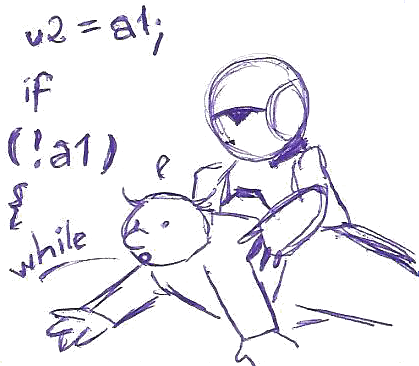
\includegraphics[scale=0.25]{images/program-extraction-without-border}}
    {\usebeamercolor[fg]{item}$\boldsymbol{\phantom{\xleftrightarrow{\qquad\quad}}}$}
    \parbox{0.25\textwidth}{\begin{center}#1\end{center}}
  \end{center}}

\setlength\parskip{\medskipamount}
\setlength\parindent{0pt}

\title{Konstruktive Mathematik, die Doppelnegationsübersetzung und Continuations}
\author{Ingo Blechschmidt}
\date{4. Dezember 2015}

\usetheme{Warsaw}
\usecolortheme{seahorse}
%\usefonttheme{default}?
%\usepackage{kurier}?
\usefonttheme{serif}
\usepackage[T1]{fontenc}
\usepackage{libertine}
%\usepackage{mathpazo}
\useinnertheme{rectangles}

\setbeamertemplate{blocks}[rounded][shadow=false]

\newenvironment{changemargin}[2]{%
  \begin{list}{}{%
    \setlength{\topsep}{0pt}%
    \setlength{\leftmargin}{#1}%
    \setlength{\rightmargin}{#2}%
    \setlength{\listparindent}{\parindent}%
    \setlength{\itemindent}{\parindent}%
    \setlength{\parsep}{\parskip}%
  }%
  \item[]}{\end{list}}

\newcommand{\pointthis}[2]{%
  \tikz[remember picture,baseline]{\node[anchor=base,inner sep=0,outer sep=0]%
    (#1) {#1};\node[overlay,rectangle callout,%
    callout relative pointer={(-0.2cm,0.8cm)},fill=blue!20] at ($(#1.north)+(1.8cm,-1.4cm)$) {#2};}%
}%

\newcommand{\hcancel}[5]{%
  \tikz[baseline=(tocancel.base)]{
    \node[inner sep=0pt,outer sep=0pt] (tocancel) {#1};
    \draw[red, line width=0.4mm] ($(tocancel.south west)+(#2,#3)$) -- ($(tocancel.north east)+(#4,#5)$);
  }%
}

\newcommand{\slogan}[1]{%
  \begin{center}%
    \setlength{\fboxrule}{2pt}%
    \setlength{\fboxsep}{5pt}%
    {\usebeamercolor[fg]{item}\fbox{\usebeamercolor[fg]{normal
    text}\parbox{0.87\textwidth}{#1}}}%
  \end{center}%
}

\setbeamertemplate{frametitle}[default][colsep=-2bp,rounded=false,shadow=false,center]
\setbeamertemplate{frametitle}{%
  \vskip1em%
  \leavevmode%
  \begin{beamercolorbox}[dp=1ex,center]{}%
      \usebeamercolor[fg]{item}{\textbf{\Large \insertframetitle}}
  \end{beamercolorbox}%
}


\setbeamertemplate{headline}{}
\setbeamertemplate{navigation symbols}{}

\newcounter{framenumberpreappendix}
\newcommand{\backupstart}{
  \setcounter{framenumberpreappendix}{\value{framenumber}}
}
\newcommand{\backupend}{
  \addtocounter{framenumberpreappendix}{-\value{framenumber}}
  \addtocounter{framenumber}{\value{framenumberpreappendix}} 
}

\setbeamertemplate{footline}{%
  \begin{beamercolorbox}[wd=\paperwidth,ht=2.5ex,dp=1.25ex,right,rightskip=1mm,leftskip=1mm]{frametitle right}
    {\quad} \inserttitle \hfill \insertauthor \quad
    \insertframenumber\,/\,\inserttotalframenumber {\quad}
  \end{beamercolorbox}}

\newcommand{\hil}[1]{{\usebeamercolor[fg]{item}{\textbf{#1}}}}

\IfSubStr{\jobname}{\detokenize{nonotes}}{
  \setbeameroption{hide notes}
}{
  \setbeameroption{show notes}
}
\setbeamertemplate{note page}[plain]

\begin{document}

\begin{frame}[c]
  \centering
  
\includegraphics[scale=0.5]{images/fortune-teller}
  \medskip

  \hil{Konstruktive Mathematik, \\ die Doppelnegationsübersetzung und Continuations}
  \medskip

  \scriptsize
  Ingo Blechschmidt \\
  Universität Augsburg
  \medskip

  Haskell in Leipzig \\
  4. Dezember 2015
  \par
\end{frame}


\section{Konstruktive Mathematik}

\subsection{Das Axiom vom ausgeschlossenen Dritten}

\begin{frame}\frametitle{Nichtkonstruktive Beweise}
  Eine Zahl heißt genau dann \hil{rational}, wenn sie sich als Bruch zweier
  ganzer Zahlen schreiben lässt.
  \begin{itemize}
    \item $\frac{21}{13}$ und $37$ sind rational.
    \item $\sqrt{2}$ und $\pi$ sind irrational.
  \end{itemize}

  \only<1>{\vspace*{1em}\centering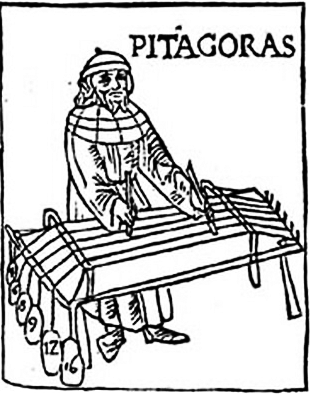
\includegraphics[scale=0.3]{images/pythagoras}}

  \pause

  \hil{Satz.} Es gibt \hil{irrationale} Zahlen~$x$ und~$y$ sodass~$x^y$ rational ist.
  \medskip

  \pause
  \hil{Beweis.} Entweder ist~$\sqrt{2}^{\sqrt{2}}$ rational oder nicht.
  \begin{enumerate}
    \item Im ersten Fall sind wir fertig.
    \item Im zweiten Fall können wir~$x \defeq \sqrt{2}^{\sqrt{2}}$ und~$y \defeq
  \sqrt{2}$ nehmen. Dann ist~$x^y = \sqrt{2}^{\sqrt{2} \cdot \sqrt{2}} =
  \sqrt{2}^2 = 2$ rational.
  \end{enumerate}
\end{frame}

\newcommand{\constructiveinterpretation}{
  \begin{minipage}{0.99\textwidth}
    \begin{block}{\centering Konstruktive Interpretation}
      \begin{description}\small
        \item[$\bot$] Widerspruch.
        \item[$A \wedge B$] Wir haben Beleg für~$A$ und für~$B$.
        \item[$A \vee B$] Wir haben Beleg für~$A$ oder für~$B$.
        \item[$A \Rightarrow B$] Wir können Beleg für~$A$ in Beleg für~$B$
        transformieren.
        \item[$\forall x{:}X\_ A(x)$] Zu jedem $x:X$ können wir Beleg für
        $A(x)$ konstruieren.
        \item[$\exists x{:}X\_ A(x)$] Wir haben ein $x:X$ zusammen mit Beleg
        für~$A(x)$.
      \end{description}
    \end{block}
  \end{minipage}
}

\frame{\frametitle{Das Axiom vom ausgeschlossenen Dritten}
  \centering
  "`Für jede Aussage~$A$ dürfen wir~$A \,\vee\, \neg A$ voraussetzen."'

  \medskip
  Klassische Logik $=$ \\
  konstruktive Logik $+$ das Axiom vom ausgeschlossenen Dritten.

  \vfill

  \only<1>{
    \centering
    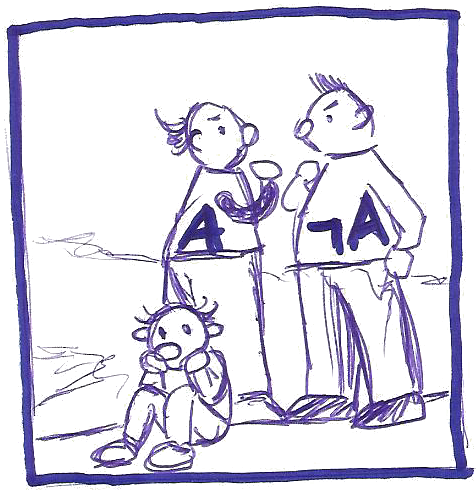
\includegraphics[scale=0.7]{images/lem}
    \par
  }

  \only<2>{
    \begin{minipage}{0.8\textwidth}
      \begin{block}{\centering Klassische Interpretation}
        \begin{description}\small
          \item[$\bot$] Widerspruch.
          \item[$A \wedge B$] $A$ und $B$ sind wahr.
          \item[$A \vee B$] $A$ ist wahr oder $B$ ist wahr.
          \item[$A \Rightarrow B$] Sollte $A$ wahr sein, so auch $B$.
          \item[$\forall x{:}X\_ A(x)$] Für alle $x:X$ gilt $A(x)$.
          \item[$\exists x{:}X\_ A(x)$] Es gibt ein $x:X$ mit $A(x)$.
        \end{description}
      \end{block}
    \end{minipage}
  }
  \only<3>{
    \vfill
    \constructiveinterpretation
  }
  \par
}

\begin{frame}\frametitle{Negierte Aussagen}
  \centering
  "`$\neg A$"' ist syntaktischer Zucker für $(A \Rightarrow \bot)$ \\[0.2em]
  und bedeutet: Es gibt keinen Beleg für~$A$.

  \vfill
  \constructiveinterpretation
  \par
\end{frame}

\begin{frame}\frametitle{Doppelt negierte Aussagen}
  \centering
  "`$\neg\neg A$"' bedeutet: Es gibt keinen Beleg für~$\neg A$.

  Aus~$A$ folgt trivialerweise $\neg\neg A$. \\
  Aber nicht umgekehrt.

  \vfill
  \only<1>{\constructiveinterpretation}
  \only<2>{
    \begin{minipage}{0.95\textwidth}
      \begin{block}{\centering Wo ist der Schlüssel?}
        \centering
        Es gibt \hil{nicht nicht} eine Stelle, an der der Schlüssel liegt.  \\[0.7em]
        \emph{versus} \\[0.7em]
        Es gibt eine Selle, an der der Schlüssel liegt.
      \end{block}
    \end{minipage}
  }
  \par
\end{frame}

\newcommand{\inegneg}{{\usebeamercolor[fg]{item}{\boldsymbol{\neg\neg}}}}
\newcommand{\gnegneg}[1]{\textcolor{gray}{\boldsymbol{\neg\neg}(}#1\textcolor{gray}{)}}

\begin{frame}\frametitle{Die Doppelnegationsübersetzung}
  \vspace*{-2em}
  \begin{align*}
%   (x=y)^\Box &\defeqv \inegneg (x=y) \\
    (A \wedge B)^\Box &\defeqv \gnegneg{A^\Box \wedge B^\Box} \\
    (A \vee B)^\Box &\defeqv \inegneg(A^\Box \vee B^\Box) \\
    (A \Rightarrow B)^\Box &\defeqv \gnegneg{A^\Box \Rightarrow B^\Box} \\
    (\forall x{:}X\_ A(x))^\Box &\defeqv \gnegneg{\forall x{:}X\_ A^\Box(x)} \\
    (\exists x{:}X\_ A(x))^\Box &\defeqv \inegneg(\exists x{:}X\_ A^\Box(x))
  \end{align*}

  Beispiel: Die Doppelnegationsübersetzung von
  \begin{center}
    \emph{Es gibt eine Stelle, an der der Schlüssel liegt.}
  \end{center}
  ist
  \begin{center}
    \emph{Es gibt \hil{nicht nicht} eine Stelle, an der der Schlüssel
    liegt.}
  \end{center}

  \hil{Satz.} Es gilt $A$ genau dann klassisch, wenn $A^\Box$ konstruktiv gilt.
\end{frame}


\section{Die Curry--Howard-Korrespondenz}

\begin{frame}\frametitle{Die Curry--Howard-Korrespondenz}
  \korr{\hil{Aussagen}}{\hil{Typen}}
  \vspace*{-3em}
  \pkorr{\usebeamercolor[fg]{item}$\boldsymbol{\Biggl|}$}{\usebeamercolor[fg]{item}$\boldsymbol{\Biggl|}$}
  \vspace*{-3em}
  \korr{\hil{Beweise}}{\hil{Terme}}

  \only<1>{
    \centering
    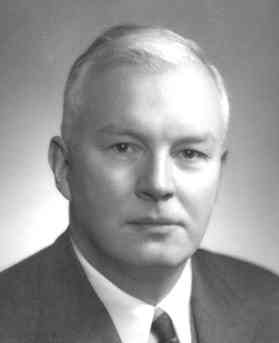
\includegraphics[height=2.2cm]{images/haskell-curry}
    \qquad
    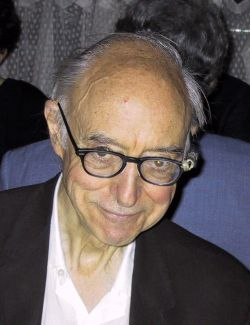
\includegraphics[height=2.2cm]{images/william-howard}
    \par
  }

  \only<2>{
    \centering
    \setlength{\extrarowheight}{0.3em}
    \begin{tabular}{l@{\qquad}l}
      \hil{Logik} & \hil{Programmierung} \\
      $A \Rightarrow A$ & \texttt{A $\to$ A} \\
      $(A \wedge B) \Rightarrow A$ & \texttt{(A,B) $\to$ A} \\
      $A \Rightarrow (A \vee B)$ & \texttt{A $\to$ Either A B}
    \end{tabular}
    \par
  }
\end{frame}

\begin{frame}\frametitle{Die Curry--Howard-Korrespondenz}
  \centering
  \small
  \vspace*{-0.5em}
  \setlength{\extrarowheight}{0.3em}
  \begin{tabular}{l@{\qquad}l}
    \hil{Logik} & \hil{Programmierung} \\
    Aussage $A$ & Typ \texttt{A} der Belege für $A$ \\
    Beweis von $A$ & Programm vom Typ \texttt{A} \\
    $A \Rightarrow A$ & \texttt{A $\to$ A} \\
    $(A \wedge B) \Rightarrow A$ & \texttt{(A,B) $\to$ A} \\
    $A \Rightarrow (A \vee B)$ & \texttt{A $\to$ Either A B} \\
    $A \Rightarrow B$ & \texttt{A $\to$ B} \\
    \text{Es gibt eine natürliche Zahl.} & \texttt{Nat} \\
    \visible<2->{$\neg A$\visible<3->{, d.\,h. $A \Rightarrow \bot$} &
      \only<2-3>{??}
      \visible<4->{\texttt{A $\to$ r}}} \\
    \visible<5->{$\neg\neg A$, d.\,h. $(A \Rightarrow \bot) \Rightarrow \bot$} &
      \only<5>{??}
      \visible<6->{\texttt{(A $\to$ r) $\to$ r}\visible<7->{, d.\,h. \texttt{Cont r A}}}
  \end{tabular}
  \par

  \slogan{
    Aus jedem konstruktiven Beweis kann man ein Programm extrahieren.
    Jedes Programm beweist eine Behauptung.
  }
\end{frame}

\begin{frame}[fragile]\frametitle{$\boldsymbol{\neg\neg}$-Übersetzung $\widehat=$ CPS-Transformation}
  \begin{changemargin}{-0.3em}{0em}
    \centering
    \vspace*{-1em}
    \setlength{\extrarowheight}{0.3em}
    \begin{tabular}{@{}l@{\qquad}l}
      \hil{Logik} & \hil{Programmierung} \\
      Aussage $A$ & Typ \texttt{A} der Belege für $A$ \\
      Beweis von $A$ & Programm vom Typ \texttt{A} \\
      $\neg\neg A$, d.\,h. $(A \Rightarrow \bot) \Rightarrow \bot$ &
        \texttt{(A $\to$ r) $\to$ r}, d.\,h. \texttt{Cont r A} \\
      Doppelnegationsübersetzung & CPS-Transformation
    \end{tabular}

    \begin{minted}{haskell}
type Cont r a = ((a -> r) -> r)

-- Axiom vom ausgeschlossenen Dritten ohne Übersetzung:
-- lem :: Either a (a -> r)

lem :: Cont r (Either a (a -> Cont r b))
lem = \k -> k $ Right $ \x -> (\k' -> k (Left x))
    \end{minted}
  \end{changemargin}
\end{frame}

\begin{frame}[fragile]\frametitle{Minima unendlicher Listen}
  \hil{Satz.} In jeder unendlichen Liste~\texttt{xs} natürlicher Zahlen gibt es
  ein kleinstes Element.

  Aber nicht konstruktiv! Es gibt kein Programm vom Typ:
  \begin{center}
    \begin{minipage}{0.7\textwidth}
      \begin{minted}{haskell}
minimum :: [Nat] -> Ix
-- Ix: Typ der Indizes (also auch Nat)
      \end{minted}
    \end{minipage}
  \end{center}

  \pause
  \hil{Beweis.} Durch Induktion über die Größe eines gegebenen
  Elements~\texttt{xs!!i}.
  \begin{itemize}
    \item Anfang: Also \texttt{xs!!i == 0}. Damit ist \texttt{xs!!i}
    minimal.
    \item Schritt: Entweder gibt es \texttt{j} mit \texttt{xs!!j < xs!!i} oder nicht.
    \begin{enumerate}
      \item Im ersten Fall gibt es ein Minimum nach Ind'voraussetzung.
      \item Im zweiten Fall ist \texttt{xs!!i} minimal.
    \end{enumerate}
  \end{itemize}
\end{frame}

\begin{frame}[fragile]\frametitle{Minima unendlicher Listen}
  \only<2>{\footnotesize\vspace*{-1.5em}}
  \begin{minted}{haskell}
type Cont r a = ((a -> r) -> r)

lem :: Cont r (Either a (a -> Cont r b))
lem = \k -> k $ Right $ \x -> (\k' -> k (Left x))

minimum :: [Nat] -> Cont r (Ix, Ix -> Cont r ())
minimum xs = go 0 where
   go i = do
      oracle <- lem
      case oracle of
         Left  j -> go j
         Right f -> return (i, \j ->
            if xs!!j >= xs!!i then return () else f j)
  \end{minted}
  \pause
  \begin{minted}{haskell}
example = do
   (i, g) <- minimum [...]
   g 5 >> g 7 >> g 3
   ...
  \end{minted}
\end{frame}

\end{document}
